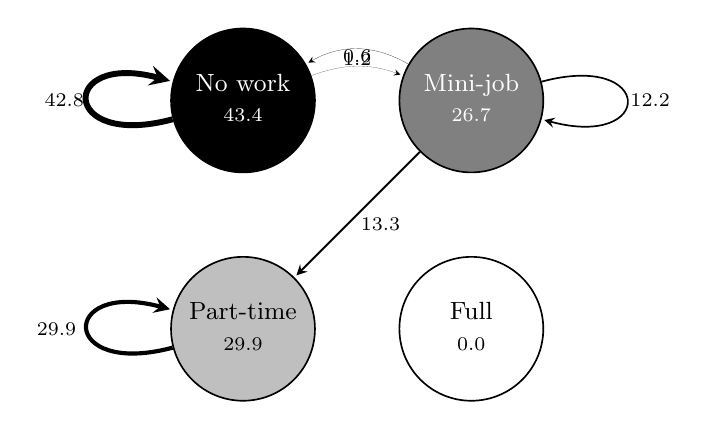
\begin{tikzpicture}[->,>=stealth,shorten >=1pt,auto,node distance=2.9cm, semithick] \tikzstyle{state}=[circle,fill=gray,draw=black,text=white]\node[state, fill=black,     minimum size=52pt, inner sep = -3pt]              (1)               {\small \begin{tabular}{c} No work  \\ {\scriptsize43.4}\end{tabular}}; \node[state, fill=gray,      minimum size=52pt, inner sep = -3pt]              (2) [right of=1]  {\small \begin{tabular}{c} Mini-job \\ {\scriptsize26.7}\end{tabular}}; \node[state, fill=lightgray, text=black, minimum size=52pt, inner sep = -3pt]  (3) [below of=1]  {\small \begin{tabular}{c} Part-time\\ {\scriptsize29.9}\end{tabular}}; \node[state, fill=white,     text=black,  minimum size=52pt, inner sep = -3pt] (4) [right of=3]  {\small \begin{tabular}{c} Full     \\ {\scriptsize0.0}\end{tabular}};\path(1) edge[line width=2.14pt,loop left,outer sep=-2pt] node {\scriptsize 42.8} (1)(1) edge[line width=0.03pt,bend left=20,outer sep=-2pt] node {\scriptsize 0.6} (2)(2) edge[line width=0.06pt,bend right,outer sep=-2pt] node {\scriptsize 1.2} (1)(2) edge[line width=0.61pt,loop right=20,outer sep=-2pt] node {\scriptsize 12.2} (2)(2) edge[line width=0.67pt,outer sep=-2pt] node {\scriptsize 13.3} (3)(3) edge[line width=1.50pt,loop left=-2pt] node {\scriptsize 29.9} (3); \end{tikzpicture} 